\documentclass[12pt,twoside,a4paper, spanish]{article}
\usepackage[spanish]{babel}
\selectlanguage{spanish}
\usepackage[utf8]{inputenc}
\usepackage{graphicx}\usepackage{graphicx}



\usepackage{geometry}
\geometry{
	a4paper,
	total={170mm,257mm},
	left=20mm,
	top=20mm,
}




\renewcommand{\baselinestretch}{1.5}

\begin{document}
	
	\title{TypeScript}
	\author{Mario Moraño Orviz \\
	Adrián Mínguez Graña \\
	Sergio Álvarez Alonso \\
	Ángel Manuel Méndez Campal}
	\date{Septiembre 2018}
	\maketitle
	
	\begin{abstract}
	Trabajo consistente en describir el lenguaje de programación Typescript y su relación en la asignatura, centrándose en al descripción sus principales características, el porqué de su creación y utilidad en el contexto de la web.
	\end{abstract}

    \section{Contexto y motivación del lenguaje}
    Se trata de un lenguaje de programación que surge en el año 2012 de la mano de Microsoft, tras dos años de desarrollo interno de la compañía. La motivación de los ingenieros de Microsoft para desarrollar dicha tecnología consiste en la demanda de muchos desarrolladores web de contar con herramientas que ayudasen a escalar sus aplicaciones. El desarrollo web en javascript no era en ese año una experiencia agradable para el programador, y el escalado de sitios web hacia aplicaciones más grandes era una tarea dificultosa debido a la naturaleza del propio lenguaje. En conclusión, el uso de javascript en la web crecía exponencialmente y también la complejidad del software producido, sin que la herramienta contase con características que se ajustasen a la demanda de los programadores. \\
    
    La solución por parte de Microsoft a dicho problema fue el desarrollo del lenguaje de programación Typescript, que permitía a los usuarios no tener que esperar a futuras versiones de ECMAScript para poder desarrollar con nuevas características de javascript, además de dotar al lenguaje con un sistema de tipado fuerte. En éste sentido se puede decir que el desarrollo de Typescript iba "por delante" de ECMAScript, y su punto fuerte es que al ser un superset de javascript, todo el código javascript es de forma automática código typescript válido, gracias al compilador TSC.
    
    \begin{figure}[h]
    	\centering
    	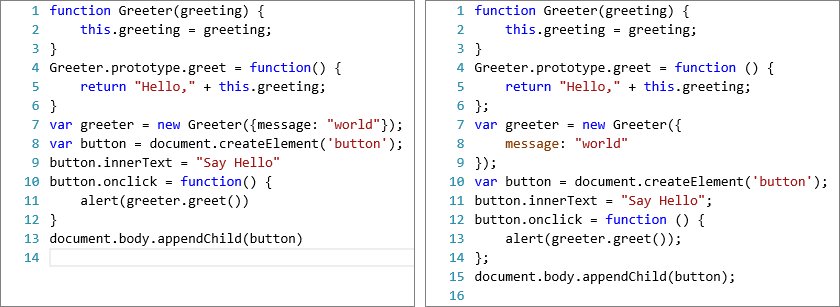
\includegraphics[width=0.8\textwidth]{imagenes/ts3.png}
    	\caption{Comparación ts vs js I.}
    \end{figure}

	Como se puede apreciar en la figura 1, el código generado al transcompilar typescript es prácticamente igual al código javascript, salvo algunas cuestiones semánticas como puntos y coma o espacios. Cabe destacar el que todo el codigo javascript es código typescript válido: sin más que renombrar el fichero .js a .ts y compilar con TSC se obtiene javascript válido. \\
	
	Ocurre que el ejemplo código anterior contiene un error que sólo será detectado por javascript en tiempo de ejecución debido al carácter dinámico del lenguaje, y no durante el desarrollo. De este modo obtendremos el siguente pop-up al ejecutarlo con un navegador:
	
	\begin{figure}[h]
		\centering
		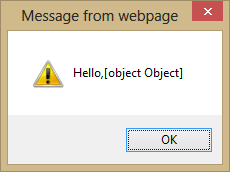
\includegraphics[width=0.5\textwidth]{imagenes/ts4.png}
		\caption{Error en t ejecución. JS dinámico}
	\end{figure}

	Con typescript se posibilita el añadir anotaciones de tipo a las variables definidas
	en el código del programa. Al introducir tipado estático la información que puede proveer el compilador y el abanico de herramientas de desarrollo disponible mejoran notablemente, proveyendo al usuario una experiencia mucho más completa que con javascript, como el hecho de disponer de mensajes en el código y detección de errores en tiempo de compilacón. Además al compilar se eliminan todas las anotaciones "de tipos", con lo que el código resultante siempre será código javascript válido.
	
	\begin{figure}[h]
		\centering
		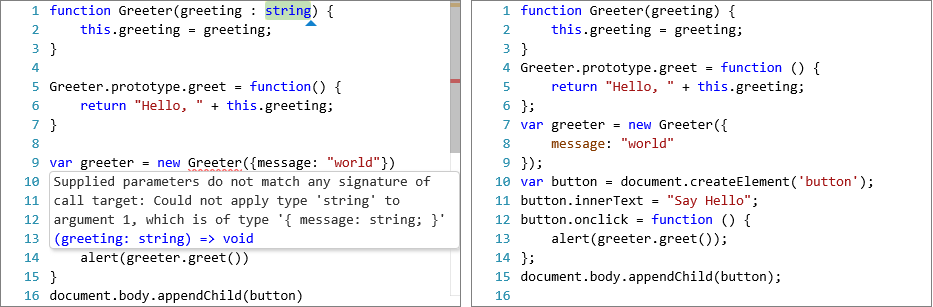
\includegraphics[width=0.8\textwidth]{imagenes/ts5.png}
		\caption{Errores inline gracias a TSC}
	\end{figure}

	Otra característica principal es su interoperabilidad con javascript. Además de continuar utilizando sus librerías, los usuarios de ts cuentan con la posbilidad de declarar crear un fichero de declaración que les permite utilizar sus característicar sin tener que modificar el código js. Ésto es útil porque permite integrar el lenguaje con IntelliSense de visual estudio y hacer comprobaciones en tiempo de compilación: uso del DOM, librerías jQuery y WinRT, etc. \\
	
	El sistema de tipos de typescript es ligero con lo que los desarrolladores no están obligados a introducir tipado en todos los componentes del proyecto al hacer una migración desde javascript. Ésto se utilizan de manera opcional en mayor medida cuanto mayor sea la necesidad del usuario de mejorar su entorno de trabajo. El compilador TSC también tiene la capacidad de inferir tipos automáticamente.
    
    \section{Principales características}
    
    Entre las principales características de typescript destacan que permite declarar clases y utilizar módulos. El nivel de encapsulación que se consigue con typescript es grande debido a que su orientación a objetos es fuerte, idea obtenida de ECMAScript 6 pero adelantándose a la release. A continuación se presenta un ejemplo de declaración de clase en typescript y el correspondiente código js generado:
    
    \begin{figure}[h]
    	\centering
    	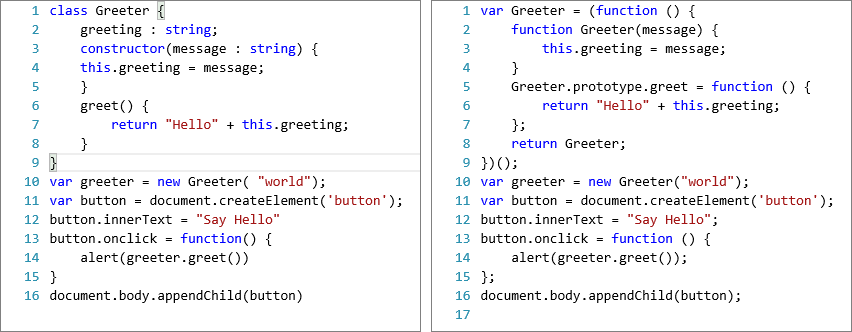
\includegraphics[width=0.8\textwidth]{imagenes/ts7.png}
    	\caption{Declaración de clase(izda) y código generado (dcha)}
    \end{figure}

	Typescript dota también de acceso a interfaces, lo cual habilita mecanismos para utilizar herencia y funcionalidad compartida de los objetos creados, además del mencionado sistema de módulos para agrupar código relacionado en espacios de nombres. Es compatible con los sistemas de cargar módulos de typescript como Commonjs, con lo que se pueden cargar en tiempo de ejecución y cargar dependencias entre ellos. Éstas y otras características de typescript dotan a los sitios web escritos en js de la capacidad de escalar a portales más grandes de forma más eficiente y segura.
    
    \section{Ejemplo de aplicación}
    
    Hemos realizado una pequeña aplicación a modo de ejemplo utilizando el framework angular, que utiliza typescript como lenguaje base para la construcción de aplicaciones. Se trata de un pequeño portal web sobre información de la NBA. Está desplegada en una de las máquinas virtuales de la escuela (ubuntu): www.moraorviz.com/angular-experimental.
    
    \section{Conclusiones y valoración}
    

	
\end{document}